% BSD 3-Clause License
%
% Copyright (c) 2023 Quux System and Technology. All rights reserved.
%
% Redistribution and use in source and binary forms, with or without
% modification, are permitted provided that the following conditions are met:
%
% 1. Redistributions of source code must retain the above copyright notice, this
%    list of conditions and the following disclaimer.
%
% 2. Redistributions in binary form must reproduce the above copyright notice,
%    this list of conditions and the following disclaimer in the documentation
%    and/or other materials provided with the distribution.
%
% 3. Neither the name of the copyright holder nor the names of its
%    contributors may be used to endorse or promote products derived from
%    this software without specific prior written permission.
%
% THIS SOFTWARE IS PROVIDED BY THE COPYRIGHT HOLDERS AND CONTRIBUTORS "AS IS"
% AND ANY EXPRESS OR IMPLIED WARRANTIES, INCLUDING, BUT NOT LIMITED TO, THE
% IMPLIED WARRANTIES OF MERCHANTABILITY AND FITNESS FOR A PARTICULAR PURPOSE ARE
% DISCLAIMED. IN NO EVENT SHALL THE COPYRIGHT HOLDER OR CONTRIBUTORS BE LIABLE
% FOR ANY DIRECT, INDIRECT, INCIDENTAL, SPECIAL, EXEMPLARY, OR CONSEQUENTIAL
% DAMAGES (INCLUDING, BUT NOT LIMITED TO, PROCUREMENT OF SUBSTITUTE GOODS OR
% SERVICES; LOSS OF USE, DATA, OR PROFITS; OR BUSINESS INTERRUPTION) HOWEVER
% CAUSED AND ON ANY THEORY OF LIABILITY, WHETHER IN CONTRACT, STRICT LIABILITY,
% OR TORT (INCLUDING NEGLIGENCE OR OTHERWISE) ARISING IN ANY WAY OUT OF THE USE
% OF THIS SOFTWARE, EVEN IF ADVISED OF THE POSSIBILITY OF SUCH DAMAGE.
%
\RequirePackage[l2tabu, orthodox]{nag}
\documentclass[%
	coverheight=210mm,
	coverwidth=148mm,
	spinewidth=17.44416mm,
	flapwidth=0mm,
	wrapwidth=0mm,
	bleedwidth=5mm,
	marklength=10mm,
	foldingmargin=true,
	markthick=0.4pt,
	markcolor=black,
	pagecolor=white,
	trimmed=false,
	trimmingcolor=white
]{bookcover}
\input{git-revision.tex}
\usepackage{hyperref}
	\hypersetup{
		bookmarks=false,
		unicode=true,
		pdfduplex={DuplexFlipShortEdge},
		pdfprintscaling={AppDefault},
		pdfpicktraybypdfsize={true},
		pdfcreator={XeLaTeX},
		pdfproducer={Quux System and Technology},
		pdftoolbar={true},
		pdftitle={四川菜谱1972重制版},
		pdfsubject={封面设计},
		pdfauthor={泥偶},
		pdfkeywords={封面},
		pdflang={zh-CN},
		pdfinfo={
			GitCommitName={\gitcommitname},
			GitCommitHash={\gitcommithash},
			GitCommitterDate={\gitcommitterdate},
			PDFBuildHost={\pdfbuildhost}
		},
		hidelinks
	}
\usepackage[zihao=5]{ctexsize}
\usepackage[quiet]{xeCJK}
\usepackage{setspace}
\usepackage{pdfpages}

\begin{document}
\begin{bookcover}


\newbookcoverpart{bg block}{%
	\setpartposx{\marklength+\bleedwidth+\flapwidth+\wrapwidth+\coverwidth-51.496bp}%
	\setpartposy{\marklength}%
	\setpartheight{\coverheight+2\bleedwidth}%
	\setpartwidth{51.496bp+\spinewidth+\coverwidth+\wrapwidth+\flapwidth+\bleedwidth}%
}%

\definecolor{warm gray 1}{cmyk}{0 0 0.01 0.1}%

\bookcovercomponent{color}{bg block}{%
	warm gray 1%
}%

\bookcovercomponent{normal}{front}{%
	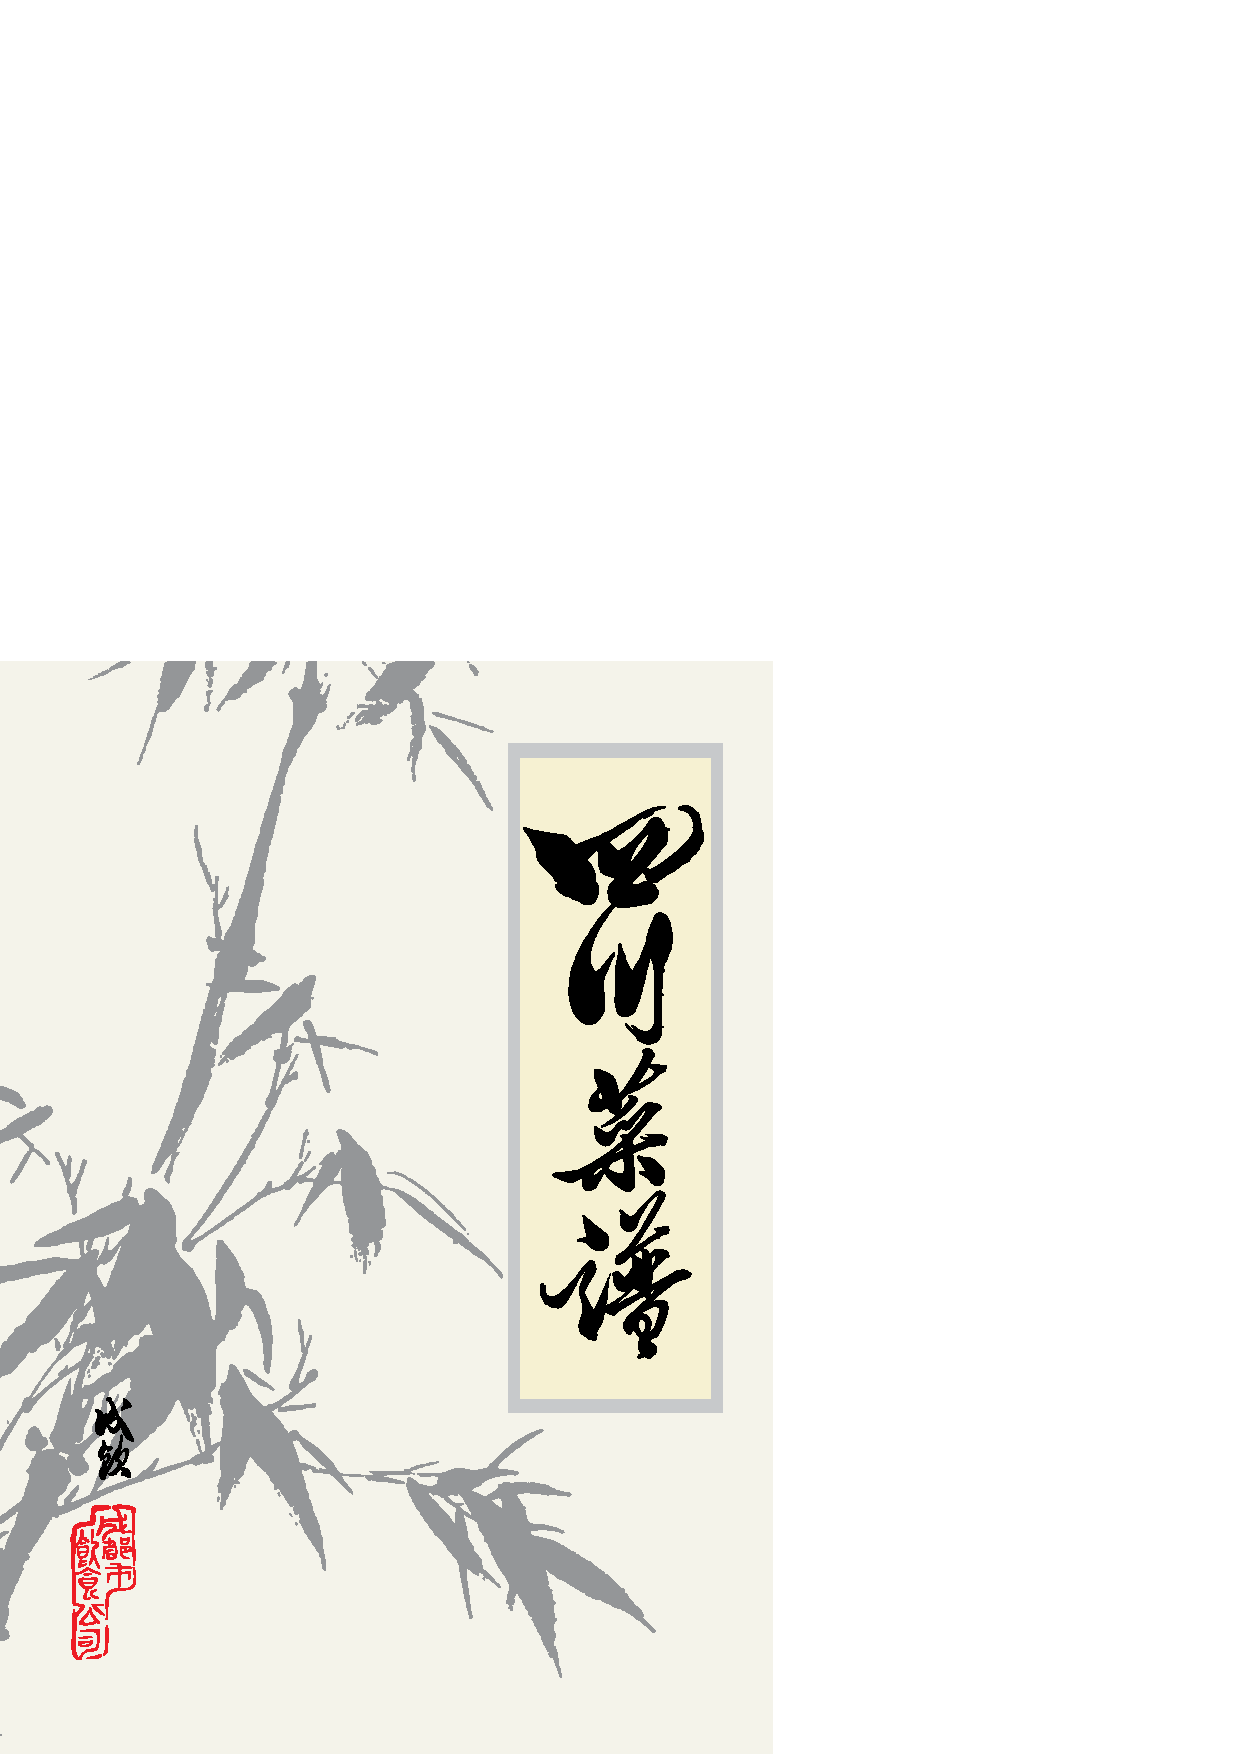
\includegraphics[page=1]{sichuan-cookbook.pdf}%
}%

\bookcovercomponent{normal}{back}{%
	\includegraphics[page=324]{sichuan-cookbook.pdf}%
}%

\bookcovercomponent{normal}{spine}{%
\singlespacing%
\setlength{\parindent}{0pt}%
\setlength{\parskip}{0\baselineskip}%
\null%

\vfill

\begin{center}
\CJKfontspec{Noto Sans CJK SC DemiLight}
\huge\sffamily%
\vspace{1\baselineskip}%
\begingroup%
\setstretch{.875}%
四\\
川\\
菜\\
谱

\endgroup%

\vspace{10\baselineskip}%

\null\hspace{2.71616pt}%

\includegraphics[height=10mm, width=10mm]{quux-logo.pdf}%
{\sffamily\tiny\kern-.5em\lower.5ex\hbox{\texttrademark}}%
\end{center}%

\vfill

\null%
}%

\end{bookcover}
\end{document}

% vim: filetype=tex noautoindent nojoinspaces
% vim: fileencoding=utf-8 formatoptions+=m
% vim: textwidth=78 tabstop=4 shiftwidth=4 softtabstop=4
